
\chapter{Impact of the choice of the correlation model}
\label{app:jets}
In this appendix we discuss the impact of different decorrelation models for the 8 TeV single-inclusive jet data
from ATLAS.
As discussed in Sec.~\ref{sec:single_jet}, these data appear to be fully consistent with the corresponding
7 TeV ones, yet they show a poor $\chi^2$ when included in the global fit.
The problem might be due to some issues in the covariance matrix of these data, in a similar way 
to what discussed in Ref.~\cite{Harland-Lang:2017ytb} for 7 TeV dataset.

%
To check whether or not this is indeed the case, starting from the default fit (\#janw) we produce two variants 
by modifying the treatment of three (out of 659) correlated systematic uncertainties
related to the jet energy scale, as suggested in Ref.~\cite{Aaboud:2017dvo}.
Specifically, in the first variation, denoted as \#janw-8dec, these three uncertainties are completely decorrelated;
in the second variation, denoted as \#janw-8pcor, they are partially decorrelated, splitting each uncertainty 
into three components and decorrelating one of them.
From Table.~\ref{tab:chi2_suppl} we see how, upon decorrelation the $\chi^2$ for ATLAS improves considerably, leaving the 
values for the other datasets almost unaffected. Very similar results are obtained when fully or partially 
decorrelating the relevant sources of systematics, thus validating the prescription of Ref.~\cite{Aaboud:2017dvo}.
At the PDFs level the results are very stable, as we see by inspection of Fig.~, where the gluon PDF for 
\#janw and \#janw-8dec are compared.

%
We conclude that the decorrelation models suggested in Ref.~\cite{Aaboud:2017dvo} solve the issue observed in
Sec.~\ref{sec:jets_res}, leading to a good fit quality of the ATLAS single-inclusive jet data at 8 TeV without
significant change in the PDFs.

\begin{table}[!t]
    \renewcommand*{\arraystretch}{1.60}
    \scriptsize
    \centering
    \begin{tabularx}{\textwidth}{Xrccc}
    \toprule
     Dataset                    & $n_{\rm dat}$ & janw &    janw-8dec   &  janw-8pcor     \\
    \midrule
     \ \ ATLAS 7 TeV            &         31  & 1.59 &  1.59 &  1.61     \\
     \ \ ATLAS 8 TeV            &        171  & 3.22 &  0.83 &  0.98     \\
     \ \ CMS   7 TeV            &        133  & 1.09 &  1.12 &  1.12     \\
     \ \ CMS   8 TeV            &        185  & 1.25 &  1.42 &  1.42     \\
     \ \ ATLAS 7 TeV            &         90  & [1.95] & [1.98] & [1.98]    \\
     \ \ CMS   7 TeV            &         54  & [2.08] & [2.19] & [2.17]    \\
     \ \ CMS   8 TeV            &        122  & [2.21] & [2.96] & [3.04]    \\
    \bottomrule
\end{tabularx}
    %-------------------------------------------------------------------------------
    \vspace{0.3cm}
    \caption{Same as Table~\ref{tab:chi2s} for
      fits performed with alternative choices of decorrelation models.
      Now only $\chi^2$ values for jet data are shown. Results for the fits with default settings
      \#janw already shown  in Table~\ref{tab:chi2s} are included for ease of reference.}
    \label{tab:chi2_suppl}
\end{table}

\begin{figure}[!t]
    \centering
    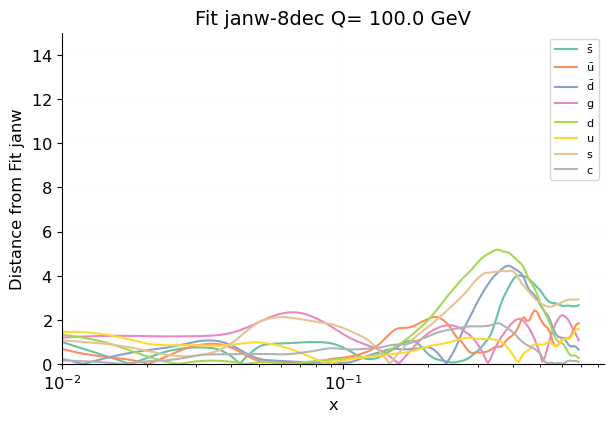
\includegraphics[scale=0.45]{distance_janw_janw-8dec}
    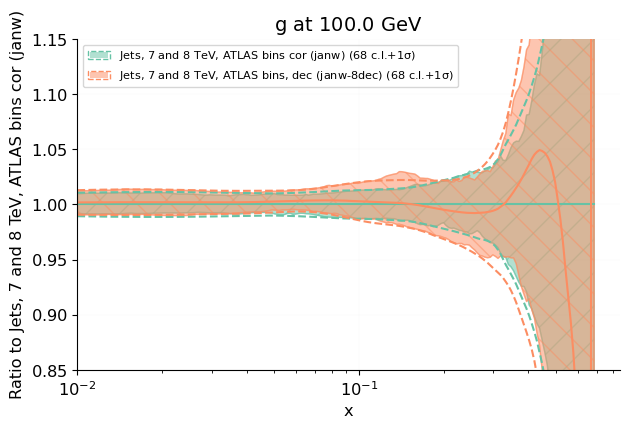
\includegraphics[scale=0.45]{jet_model_8TeV}\\
    \caption{Same as Fig.~\ref{fig:jet_data_total}, but now comparing
      the default fit to single-inclusive jet data (fit \#janw), to a fit in which selected systematic uncertainties
      are decorrelated in the ATLAS 8~TeV data (fit \#janw-8dec). The gluon is  shown as ratio to the former fit.}
    \label{fig:jet_data_model_8TeV} 
\end{figure}